\documentclass[twocolumn]{article}
\usepackage{fullpage}
\usepackage{graphicx}
\usepackage{hyperref}

\title{CS250: An Elliptic Curve Cryptography Engine}
\author{Palmer Dabbelt and Kevin Linger}
\date{December 18, 2013}

\begin{document}
\maketitle

For our CS250 project, we implemented an elliptic curve cryptagraphy
engine that attaches via the Rocket coprocessor interface.  Our
accelerator was targeted at supporting the elliptic curve digital
signature algorithm (ECDSA), a NIST standard widely used on the
Internet for digital signatures.  We built off of previous work by
doing a more involved design-space exploration, focusing on
hardware/software co-tuning. We were succesful in implementing the
primary operation needed in ECDSA which is an elliptic curve point 
multiplication. A simulated version of the operation works with the
Rocket Core, but the full toolchain did not run. With some algorithmic
improvements to our accelerator, we can get tremendous improvements
over a software implementation.

\section{Elliptic Curve Cryptography}

Digital signature algorithms\cite{fips-186-3} are a widely used class
of algorithms that are central to the functioning of the modern
Internet.  DSA\cite{us-dsa} (the original digital signature algorithm
as standardized by NIST) is a specialization of the ElGamal signature
scheme\cite{elgamal-sig} that uses discrete logarithms over finite
integer fields.  Finite integer fields are particularly easy to
compute with electronics, so this gives DSA the advantage of being an
efficient signature algorithm.

The problem is that the discrete logarithm problem is not particularly
strong over finite integer fields (specifically, there are known
sub-exponential algorithms\cite{adleman-subexp}).  As shown in
Table~\ref{key-sizes}, DSA does not scale well to higher security
levels.  This is important because code breaking algorithms are
getting more efficient, leading to the need for higher security
levels, therefore imposing higher computational costs on every node in
the system. 

\begin{table}[h]
  \begin{center}
    \begin{tabular}{cccc}
      Security Level & DSA & ECDSA & Ratio \\
      \hline
      80 & 1024 & 160 & 3:1 \\
      112 & 2048 & 224 & 6:1 \\
      128 & 3072 & 256 & 10:1 \\
      192 & 7680 & 384 & 32:1 \\
      256 & 15360 & 521 & 64:1 \\
    \end{tabular}
  \end{center}

  \caption{Comparison of DSA and ECDSA\cite{nsa-case_for_ecc}
    \label{key-sizes}}
\end{table}

The commonly accepted solution to this problem is to change the field
from integers to elliptic curves, which (as shown in
Table~\ref{key-sizes}) scale much better to higher security levels.
While elliptic curves are significantly more difficult to build
electronics for, this will eventually be offset by sheer key size
alone.  The currently accepted security level is 128 bits, at which
ECDSA already has a 10:1 advantage in key size.  Shortening the key 
size becomes even more important, as we approach a world in which 
ubiquitous embedded systems must be able to securely transmit and 
receive data.

In addition to providing for faster cryptographic operations, this
shortened key size plays an important role specific to the swarm
related to key generation.  It is already known\cite{halderman-shared}
that we can't find sufficient entropy to generate RSA-style keys for
the machines we have, much less for a network the size of that
enviosned by the swarm project.  The main problem with generating RSA
keys is finding enough entropy to search for large prime numbers, a
problem that goes away with ECDSA because the numbers are smaller and
there's no necessity for them to be prime (there is an acceptability
criteria, but the chances of a random number not meeting it are
exceedingly low).

\section{The Swarm}

One particularly interesting application of public-key cryptograhpy
arose as part of the SwarmOS project, which was the original
motivation for this accelerator.  The SwarmOS is designed to be an
operating system for the swarm, which consists of a large number
($10^{10}$) of low-powered ($\mu$W) devices as well as a smaller
number of more powerful servers.

One component of the SwarmOS is the Universal Dataplane, which is
designed to serve as a combined communication and storage mechanism
for swarm devices.  The general idea is that data will be put into the
dataplane in one place by sensors, and can then be removed anywhere
else in the world by users.  This involves a significant amount of
data being between untrusted servers, and as such the stance we
decided to take was to sign and encrypt all data all the time.

Unfortunately, ECDSA requires a significant amount of energy to
perform each signature operation (encryption is less scary because you
can cheat a bit like PGP does) -- software ECDSA is mJ per signature,
which leads to very low bandwidth on a $\mu$W machine.  The only way
to get the required $1000\times$ energy per operation improvement is
to implement ECDSA in hardware, which is essentially what this project
is.

\section{Elliptic Curve Arithmetic}

The computate-intensive operation in ECDSA is an elliptic curve (EC)
point multiplication. An EC multiply is a series of EC doubles and
additions, which are much different than the respective integer
operations. These operations are defined geometrically; e.g. to double
a point on an EC, a tangent line at that point is drawn which will
intersect the curve at exactly one other point. The result of the
double operation is that intersection point reflected over the X-axis.
An example of the geometric definition of point addition is shown in
Figure~\ref{point-add-graph}, obtained from Certicom, which involves 
drawing a line between two points on the curve, tracing its intersection with the curve, and then a reflection over the X axis -- point doubling is almost exactly
the same, except with a tangent instead of a line between the two
points (you can think of the tangent like the limit of a line between
two points as those two points approach each other).

\begin{figure}[ht]
  \begin{center}
    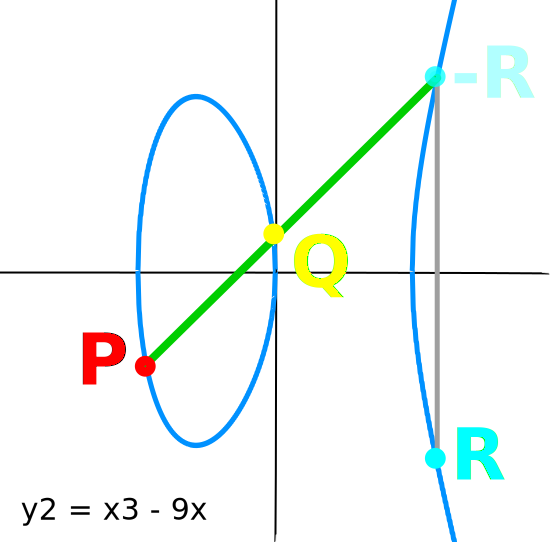
\includegraphics[width=0.9\linewidth]{point_add.svg}
  \end{center}

  \caption{Graphical definition of point add
    \label{point-add-graph}}
\end{figure}

The point add operation is described by the equation shown in
Figure~\ref{point-add-eq}, and the point double operation is described
by the equation shown in Figure~\ref{point-dub-eq}.  In these
equations all operations are modulo the order of the curve, which is
the same order of magnitune of the prime modulus of the curve (but
it's a different number).  Additionally, the curve constant $a$ is as
defined by NIST.

\begin{figure}[ht]
  $$ \lambda = \frac{P_y - Q_y}{P_x - Q_x} $$
  $$ R_x = \lambda^2 - P_x - Q_x $$
  $$ R_y = \lambda(P_x - R_x) - P_y $$

  \caption{Point addition formula
    \label{point-add-eq}}
\end{figure}

\begin{figure}[ht]
  $$ \lambda = \frac{3 * P_x^2 + a}{2P_y} $$
  $$ R_x = \lambda^2 - P_x - Q_x $$
  $$ R_y = \lambda(P_x - R_x) - P_y $$

  \caption{Point double formula
    \label{point-dub-eq}}
\end{figure}

Each of these operations also has a modular operation at the end,
where the modulus is a large prime number that represents the order of
the curve. This makes multiplication and division much more difficult:
in an accelerator where an addition takes two cycles, a modular
multiply will take on the order of a thousand cycles\cite{kss-ecdsa}.
A division is now a modular inverse followed by a modular
multiplication.

It is possible formulate the discrete logarithmic problem over
ellitic curves by repeating addition as described above.  Under
standard hardness assumptions, this formulation of the discrete
logarithm problem is assymetric (actually, this is one of the
standard hardness assumptions).  The general idea is simple: point multiplication is defined as repeated addition.  Without point doubling, for an $N$-bit
number we would have to repeat addition $O(2^N)$ times in order to do
a multiplication.  Having a formula for point doubling allows us to
reduce this to $O(N)$ point doubles along with $O(N)$ point adds by
storing some intermediate calculations along the way, just like the
long multiplication algorithm tought in grade school.  There is no
point-halving operation, so performing the inverse of a point
multiplication still requires $O(2^N)$ operations -- that's where the
assymetry comes from.

The full ECDSA algorithm essentally consists of doing a point
multiplication to generate the private and public keys -- the private
key is a random integer and the public key is that integer multiplied
by a well-known point, known as the generator point.  The remainder of
ECDSA consists of a few mathematical operations that generate enough
information to verify a signature (shown in Figure~\ref{ecdsa-sign}),
and then the inverse of that operation to verify a signature (shown in
Figure~\ref{ecdsa-verify}).  In these figures, ``$*$'' is a point
multiplication, while ``$\times$'' is a modular multiplication --
there is about a factor of $1000$ speed difference between the two.

\begin{figure}[ht]
  \begin{center}
    \includegraphics[width=0.7\linewidth]{ecdsa_sign.uncrop.pdf}
  \end{center}

  \caption{ECDSA Signature Algorithm
    \label{ecdsa-sign}}
\end{figure}

\begin{figure}[ht]
  \begin{center}
    \includegraphics[width=0.7\linewidth]{ecdsa_verify.uncrop.pdf}
  \end{center}

  \caption{ECDSA Verification Algorithm
    \label{ecdsa-verify}}
\end{figure}

Due to the large difference in complexity the point multiplication
algorithm and the remainder of the operations, the main focus of
building a fast ECDSA implementation is building a fast point multiplier

The EC point multiplication is essentially a hierarchy of control
logic that has the integer aritmetic at the base. This was the
motivation of the hardware/software cotuning: at what level of the
hierarchy should the hardware/software division be made?

\section{Implementing ECDSA}

Unlike finite integer fields, elliptic curves do not map directly to
the hardware present in current microprocessors\cite{kss-ecdsa}. This
suggests that a hardware accelerator designed to compute over elliptic
curves should lead to a significantly more efficient implementation
than in software alone.  ECDSA requires more computation per bit than
DSA, so a hardware accelerator is necessary to fully take advantage of
the smaller key size.

Previous projects\cite{nnll-ecdsa_hw} have shown that ECC hardware can
be implemented efficiently, but were limited in the amount of
design-space exploration that was attempted.  \cite{mmm-hw_ecc}
explored the tradeoffs of different algorithms for computation, but
did not explore the design space of any particular algorithm, which
seems to be the extent of the design space exploration performed.  In
addition, the current state of the art appears to consist solely of
FPGA implementations.  Unfortunately these studies don't present power
numbers, which is problematic because energy is the main limiting
factor for swarm applications.

Figure~\ref{ecdsa-sign} shows a flowchart for the signing operation
and Figure~\ref{ecdsa-verify} shows a flowchart for the verification
operation.  Both of these operations are dominated (approximately
$99.9\%$ of the runtime) by the point multiplication blocks.  As such,
most of the effort of this project was spent building a point
multiplication block.  That said, point multiplication involves
repeating point doubling and addition, which themselves involve
repeating modular multiplication and inversion.

\section{Software Test Bench}

The primary goal of this project was to explore the tradeoffs involved
in adding different amounts of hardware support for ECDSA to a
pre-existing chip.  In order to achieve this, we needed to have the
ability to generate a myriad of different software configurations that
coorespond to each of the accelerator instances we generated.

The current industry standard cryptographic software, OpenSSL, is very
difficult to hack on.  Instead of messing around with OpenSSL, we
decided to instead write our own implementation of ECDSA with the
explicit goal of being paramaterizable.  We could then generate an
instance of this software that cooresponds with every accelerator
configuration that made sense and fully test our hardware.

Unfortunately, this software implementation proved to be the weakest
point of this entire project.  As shown in Table~\ref{results}, our
code is hundreds of times slower than OpenSSL -- this is after a
significant amount of tuning, our first implementations were hundreds
of thousands of times slower than OpenSSL!  This trouble can be
attributed to two shortcommings: algorithms and tuning.

OpenSSL uses a number of significantly more complicated cryptographic
operations than our code does.  Specifically, it uses a projective
point representation that allows for the conversion of a large number
of modular inversions to a single inversion at the end of the
multiplication.  Implementing these algorithmic improvements should
show significant speedups for both our software and hardware, so it's
not entirely a bad thing.  We estimate about a $20\times$ gain can be
had from algorithmic improvements alone!

In addition to using better algorithms, OpenSSL is implemented better
than our software was.  Specifically, OpenSSL contains hand-tuned
assembly for a number of critical paths that compilers appear to
generate bad code for (specifically thinking of carry chains for
big integer operations).  Part of the problem that our implementation
had was probably related to the fact that it attempts to be
paramaterizable, which almost certainly defeats a lot of compiler
hueristics (It would be great to tell a compiler to generate 4 different
optimized versions of a function, sweeping arcoss the 4 different
values that one particularly interesting input can have).

Despite these shortcomings, we don't believe that the software troubles
completely invalidate the results from this project.  We spent about
the same amount of time on both the software and hardware. 
More importantly, we have numbers comparing
against the full-strength OpenSSL code running on x86 (a platform that
OpenSSL is highly optimized for\cite{kasper-openssl_ecc}).  These
numbers are probably the most reasonable to compare our ASIC
implementation against, as they're the most realistic picture of the
current state of the art.

\section{ASIC Implementation}

The ASIC implementation used the same algorithms as the software
implementation, and as such looks very similar.  Most ASICs end up
being limited by memory bandwidth, but ECDSA is so computationally
expensive we're not even close to being bandwidth limited (we move
roughly one bit per thousand cycles).  This has the very nice property
of allowing us to completely ignore memory, which means that the
accelerator RTL ends up looking shockingly similar to the software
implementation.

Our coprocessor interface is very simple -- essentially we relied on
the fact that almost no data was moved to avoid building anything
complicated.  A block diagram of the interface is shown in
Figure~\ref{coproc}.  The general idea is that the coprocessor has two
source registers, A and B and one destination register, C.

The host writes the data it would like to have computed to the source
registers by emiting a copy instruction a number of times (depending
on the size of the data type).  The host then emits an assembly
instruction that signifies what sort of operation it would like done.
The accelerator's control logic then sequences the functional units in
the appropriate order, eventually writing back the result to the
destination register.  The host can then emit assembly instructions to
read the results back -- if the host emits a read operation too early
it will block until the results are ready.

\begin{figure*}[t]
  \begin{center}
    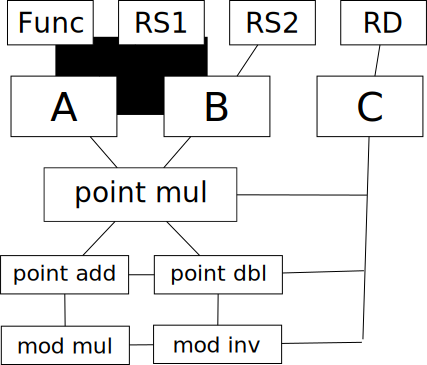
\includegraphics[width=0.5\linewidth]{coproc.svg}
  \end{center}

  \caption{Rocket Coprocessor Interface
    \label{coproc}}
\end{figure*}

While this coprocessor interface has very high overhead, it turns out
that our software implementation was sufficiently bad that doing any
fine-grained accelerator operations ended up being pointless because
of the software overhead (in addition to the interface overhead).  For
the interesting configurations the interface was very low overhead so
it didn't end up causing too much trouble.

Our ASIC implementation of ECDSA performs all elliptic field arithmetic,
including point multiplication, addition, doubling, as well as modular
multiplication and modular inversion. Our hardware supports key sizes
up to 256 bits, as that is the suggested security level.

We created instructions to expose each of the operations listed
above. Operands are pushed 64-bits at a time. We opted to have
operands pushed over the two 64-bit buses instead of having the
accelerator fetch operands from memory. This primarily comes at the
cost of register space in the rocket core, as it only takes
four to twelve instructions to push all operands to the
accelerator. In addition to setting the operands, the elliptic curve
parameters must also be sent. This is 256 bits for the modulus of the
curve, and 256 bits for the "a" parameter of the curve, which is
needed for the point doubling operation. Once a curve is set, it will
most likely be used many times, so this extra overhead of four
instructions is also negligible.

One of the biggest challenges in hardware was making sure that the
result of each operation did not exceed the modulus. This means that
on each addition becomes an add, a comparision, and potentially a
subtraction. The modular multiplication then also consists of repeated
addition and shifting instead of a large multiply followed by repeated
subtraction of the modulus. The paths with the largest propogation
delay have full adder cells, and it is likely due to the
add-check-subtract operation with 256-bit fields, which is used
numerous times throughout the functional units. This limits the clock
period to 3.5 ns. It is not obvious how to best pipeline this due to
the nature of the design, as there would be a tremendous cost in
pipeline registsrs, but it should be explored in the future.

Currently, we only have a simulated version of the rocket interface
working correctly.  We have not been able to get the compilation of
our interface with the rocket to correctly compile into Verilog
code. It is unclear why the C++ backend works in this case while the
Verilog does not.

Our hardware was written using Chisel. Verilog code was generated from
Chisel and run through the Synopsys tool flow using a 32nm educational
standard cell library. Multi-threshold cells were used, which cut the
power numbers nearly in half.

\section{Benchmarking Methodology}

Currently, we only have a simulated version of the rocket interface
working correctly.  We have not been able to get the compilation of
our interface with the rocket to correctly compile into Verilog code.
This means we couldn't actually run full signing tests through
primetime to get power numbers.  Instead we got ballpark power numbers
by running the software stack through Spike with a simulator
coprocessor to count the number of operations performed.  We then
measured the power of each operation (either Rocket integer operations
or accelerator operations) with primetime, and summed up the total.

While this isn't the greatest result, it should give us reasonable
accurate power numbers because of our algorithm.  Essentially here
we're relying on the fact that our algorithm never touches memory,
which is what allows us to assume that the Rocket core will use a
predictable amount of power.

The one big problem with this methodology is that it neglects the
power used moving data between Rocket and the coprocessor -- it just
treats these cycles as a regular integer operation.  Lucikly, for any
of the interesting configurations listed in the results section, this
overhead should be minimal -- easily within $0.1\%$.  This is
essentially because our software ECDSA implementation is so bad that
the number of cycles run by Rocket whenever we are doing anything in
software dwarfs the number of cycles moving data.  Thus, even if
moving data between Rocket and the coprocessor is very expensive
relative to moving data within a Rocket core, it won't make much of a
difference in the final power results.

\section{Results}

\begin{table}[ht]
  \begin{center}
    \begin{tabular}{c|ccc}
      Platform        & Power & Speed  & Area \\
                      & mJ/op & op/sec & mm$^2$ \\
      \hline
      OpenSSL (45nm)  & 20    & 1000   &      \\
      x86 (45 nm)     & 4000  & 5      &      \\
      Rocket          & 800   & 0.05   &      \\
      Virtex 2 (90nm) & 4000  & 250    &      \\
      Virtex 6 (45nm) & 500   & 4000   &      \\
      \hline
      Mod Mul         & 200   & 0.3    & 0.04 \\
      Mod Mul+Div     & 2     & 20     & 0.10 \\
      Point Add+Dbl   & 0.5   & 100    & 0.31 \\
      Point Mul       & 0.06  & 400    & 0.35 \\
    \end{tabular}
  \end{center}

  \caption{Comparision of results to previous work
    \label{results}}
\end{table}

Table 2 shows a comparison of our work to previous FPGA implementations, as well
as the design space exploration of having different functionality in the hardware 
and software. 

One important result to note is that certain blocks make sense to pair up in hardware. For example, a lot is gained from having modular multiplication and inversion in hardware as opposed to a single one. If the ECDSA algorithm is thought of as a hierarchy, then it can be seen that all layers in a hierarchy should be in hardware or none of them should be. 

Another result is that it does it costs a significant amount to jump from the base of the hierarchy (multiply and invert), to the elliptic curve point and add layer. Add and double are complicated control blocks with many adders, and the area of the chip is tripled. However, to move from the add and double layer to the multiply layer, there is very little cost in area for a large improvement in energy/op. When the full point multiply is put in hardware, we start to approach the $\mu$J/op territory that would desired for devices on the SwarmOS. With algorithmic and micro-architectual improvements, we will be even closer. 

\section{Future Work}

Due to time constraints, there are many useful improvements that could
be made to our accelerator. Elliptic field arthimetic is not an easy
concept to grasp, and we had to make due with using only basic
algorithms. One improvement that could be made on the ellipic field
arthimetic is transforming a two-dimensional point into a
three-dimensional represenation for point multiplication. In this
case, only one modular inversion is needed for the entire point
multiplication (as opposed to hundreds). This further might make it
unnecessary for an inversion hardware unit to be needed at
all. Another improvement is to use Montgomery
Multiplication\cite{mmm-hw_ecc}. This is a complex algorithm that
performs successive multiplications fast after some intial
overhead. If these algorithmic enhancements were made we would surely
see a tremendous speedup. Both of these improvements have interesting
time/space tradeoffs for hardware implementations, so could serve as
additional design points for our accelerator.

A primary concern should be getting our software
implementation up to snuff -- this almost certainly means adopting
OpenSSL as our testbench, hand-tuning its assembly for RISC-V, and
then modifying it to be easily paramaterizable so it can target our
family of accelerators. We will then have to modify our hardware 
implementation to take into account the algorithmic improvements that 
OpenSSL brings.

In addition to algorithmic improvements, there are a number of tricks
one can play to squeeze performance out of ECDSA.  The most important
one appears to be to build hand-crafted routines for operating on
particular curves -- for example, a mod routine for NIST's $p256$
curve is hundredes of times faster than a generic
one.

There are a number of architectural improvements that can be made to
our coprocessor interface that can help mitigate the large overhead
involved -- either placing the accelerator closer to the pipeline or
moving more state into the accelerator.  Both of these lower the
round-trip CPU to accelerator overhead and make some smaller
accelerators possible, thus providing more interesting design points.

There are also a number of interesting micro-architectural
improvements that can be made to our accelerator.  We only have a
300MHz clock, which seems exceedingly slow for what should be a
critical path of a single 256-bt adder.  Almost certainly what
happened was that there are actually two adders on the critical path,
as there are cases where one step of an algorithm requires two
additions back-to-back.  Tweaking these state machines should provide
an interesting trade-off between speed and power usage: essentially
the higher clock rate will keep more transistors toggling, they just
will not all be doing useful work.

Finally, a number of benchmarking improvements that would be
interesting to see done.  Specifically, it would be good to see a
full-system benchmark running with our accelerator attached.  This
would be particularly interesting because it would allow for some
degree of parallelism to be exposed by our accelerator to the
benchmark.  This could be very interesting because we may be able to
provide light-weight accelerator contexts (compared to POSIX threads),
which could result in an interesting userspace wrapper.

Another interesting aspect to explore would be an improved coprocessor
interface.  It's possible that there could be a very light-weight
accelerator that could provide significant energy-per-op improvements
without requiring much overhead.  Unfortunately we don't think it will
be possible to build this with the ROCC interface because of the
inherent latency involved.

CS250 was a great course for learning how to design VLSI chips using
the toolchain. It was difficult learning a new programming language to
construct hardware while also learning how to work with the VLSI
toolflow. This could have been assisted with better tutorials on
Chisel, specifically with tutorials on writing test harnesses for both the C++
simulator and more importantly the Verilog backend.

It would also have been helpful if instead of giving us ready-made
directories and skeleton code in the early labs we were given
step-by-step instructions on how to make a Chisel project from scratch
and convert it to C++ and Verliog, because we mostly ended up hacking
the the labs in really ugly ways with our accelerator to push it
through the toolflow.

\bibliographystyle{plain}
\bibliography{bibliography}

\end{document}
